\documentclass[a4paper,10pt,oneside]{book}

% packages 
\usepackage{arsclassica}    % fancy layout
\usepackage[english]{babel}\addto{\captionsenglish}{\renewcommand{\bibname}{References}}
\usepackage{caption}         % figure captions
\usepackage[square,numbers,super,sort&compress]{natbib}  % bibliography style
\usepackage[cc]{titlepic}    % enable logo on title page
\usepackage{graphicx}       % logo related

\usepackage{standalone}

% bibliography
\bibliographystyle{../thesis}

% title setup
\title{ \vspace{3in} Unravelling higher order genome organisation {\small [working
    title]} \\ \vspace{2em} {\large {\bf Results 5: Collaborations}} }
\author{Benjamin L. Moore}
\titlepic{\vspace{2.2in} 
\includegraphics[width=\textwidth]{/Users/benmoore/hvl/1yrReport/figs/igmm.png}}

\begin{document}

\maketitle

\chapter{Local chromatin conformation}

\section{Introduction}

The Hi-C assay provides a genome-wide overview of chromatin conformation, however this broad scope imposes resolution limits inherent to an all-vs-all assay. For a closer look at chromatin conformation within a region of interest, alternative C-based assays such as 3C, 4C and 5C can be employed alongside classical microscopy techniques like FISH.

Here I discuss two collaborative projects involving the use of 4C-seq and 5C data to "zoom in" on two well-studied regions related to limb development: the ZRS enhancer and HoxD gene cluster.

\section{4C of the ZRS enhancer}

% Adam sent a powerpoint he gave for section meeting, see also Prof Hill's publications

\subsection{Assay diagnostics}

\subsection{4C / Hi-C comparison}

\subsection{3D modelling}

\section{5C in the HoxD region}

% files for this under iain on ext HD
% relevant publications: http://dev.biologists.org/content/139/17/3157.full.pdf+html


\subsection{Differential contacts}

% raw diff: fold change?

\begin{figure}
\begin{center} 
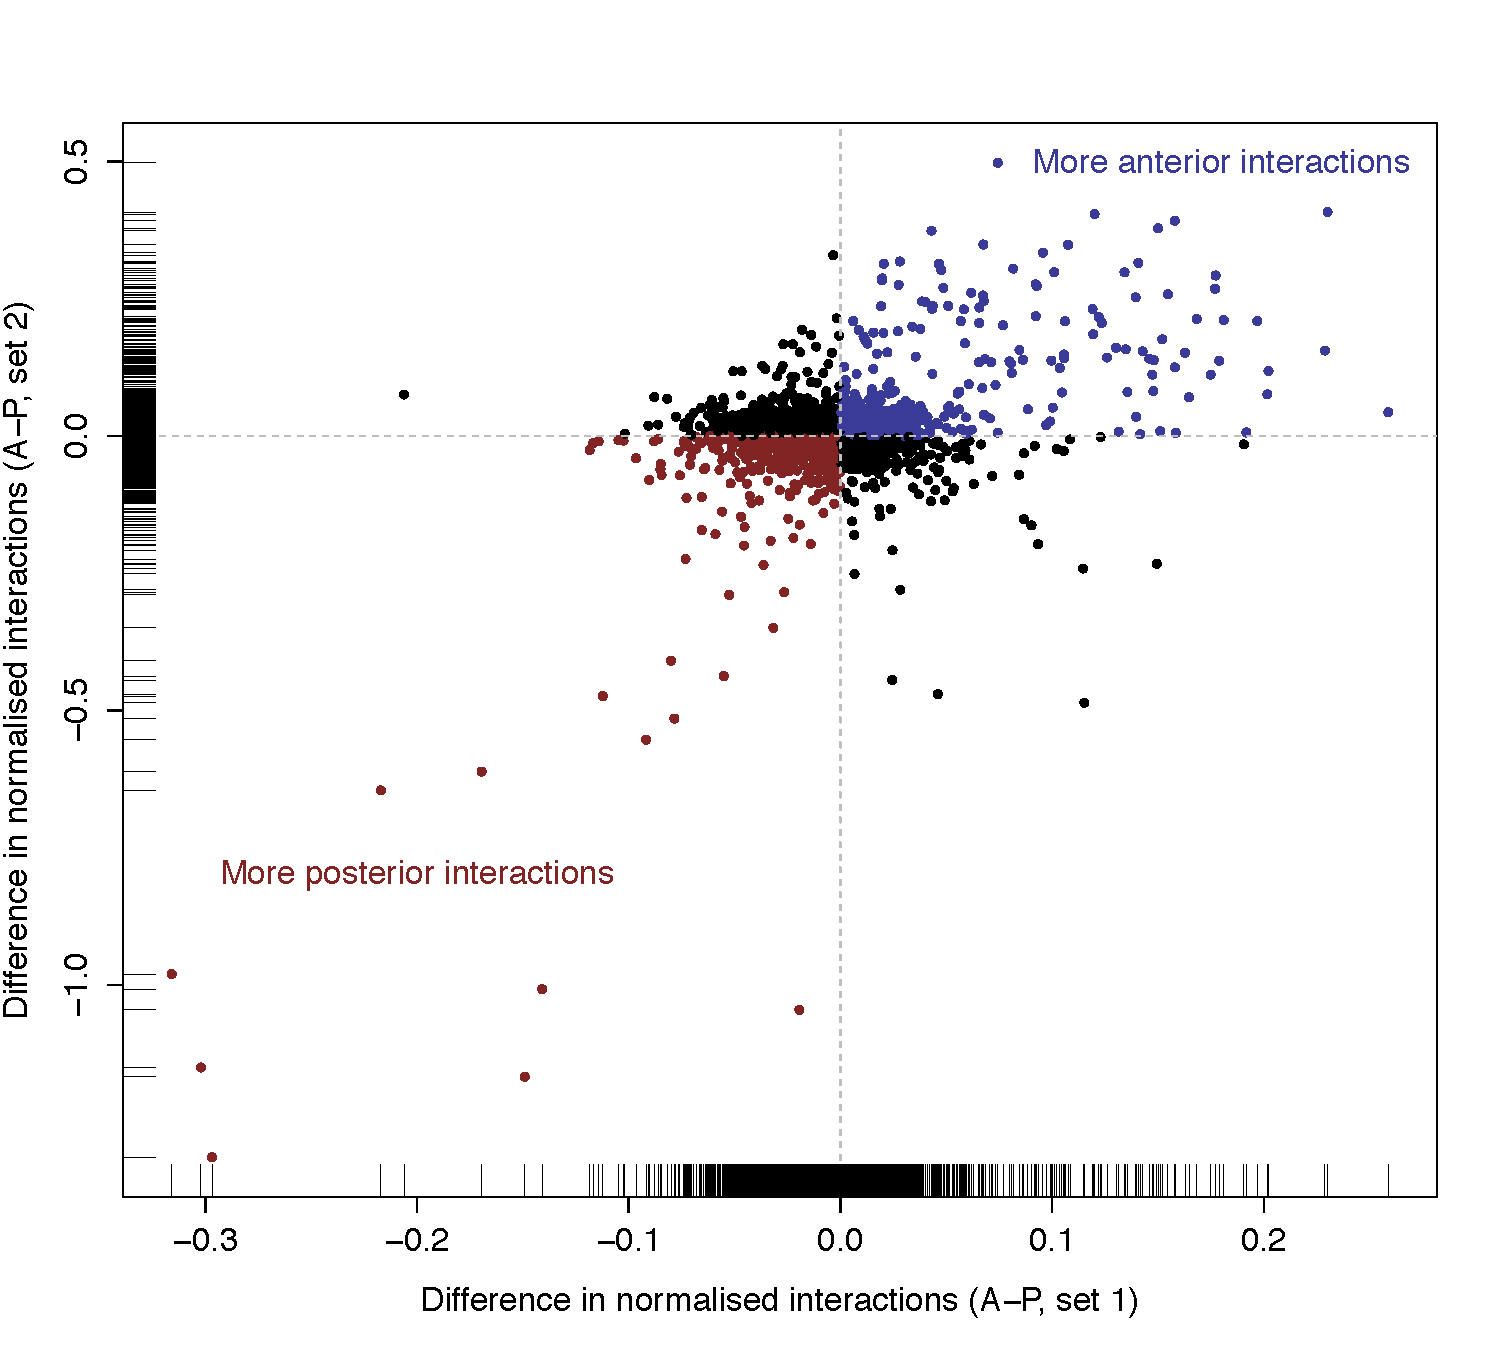
\includegraphics[width=\textwidth]{figs/5cfc.pdf}
\captionsetup{width=\textwidth} 
\caption{ {\bf Will we use this stuff? }
Placeholder
}\label{fig:5cfc}
\end{center} 
\end{figure} 

% statistical test of differential contacts

\begin{figure}
\begin{center} 
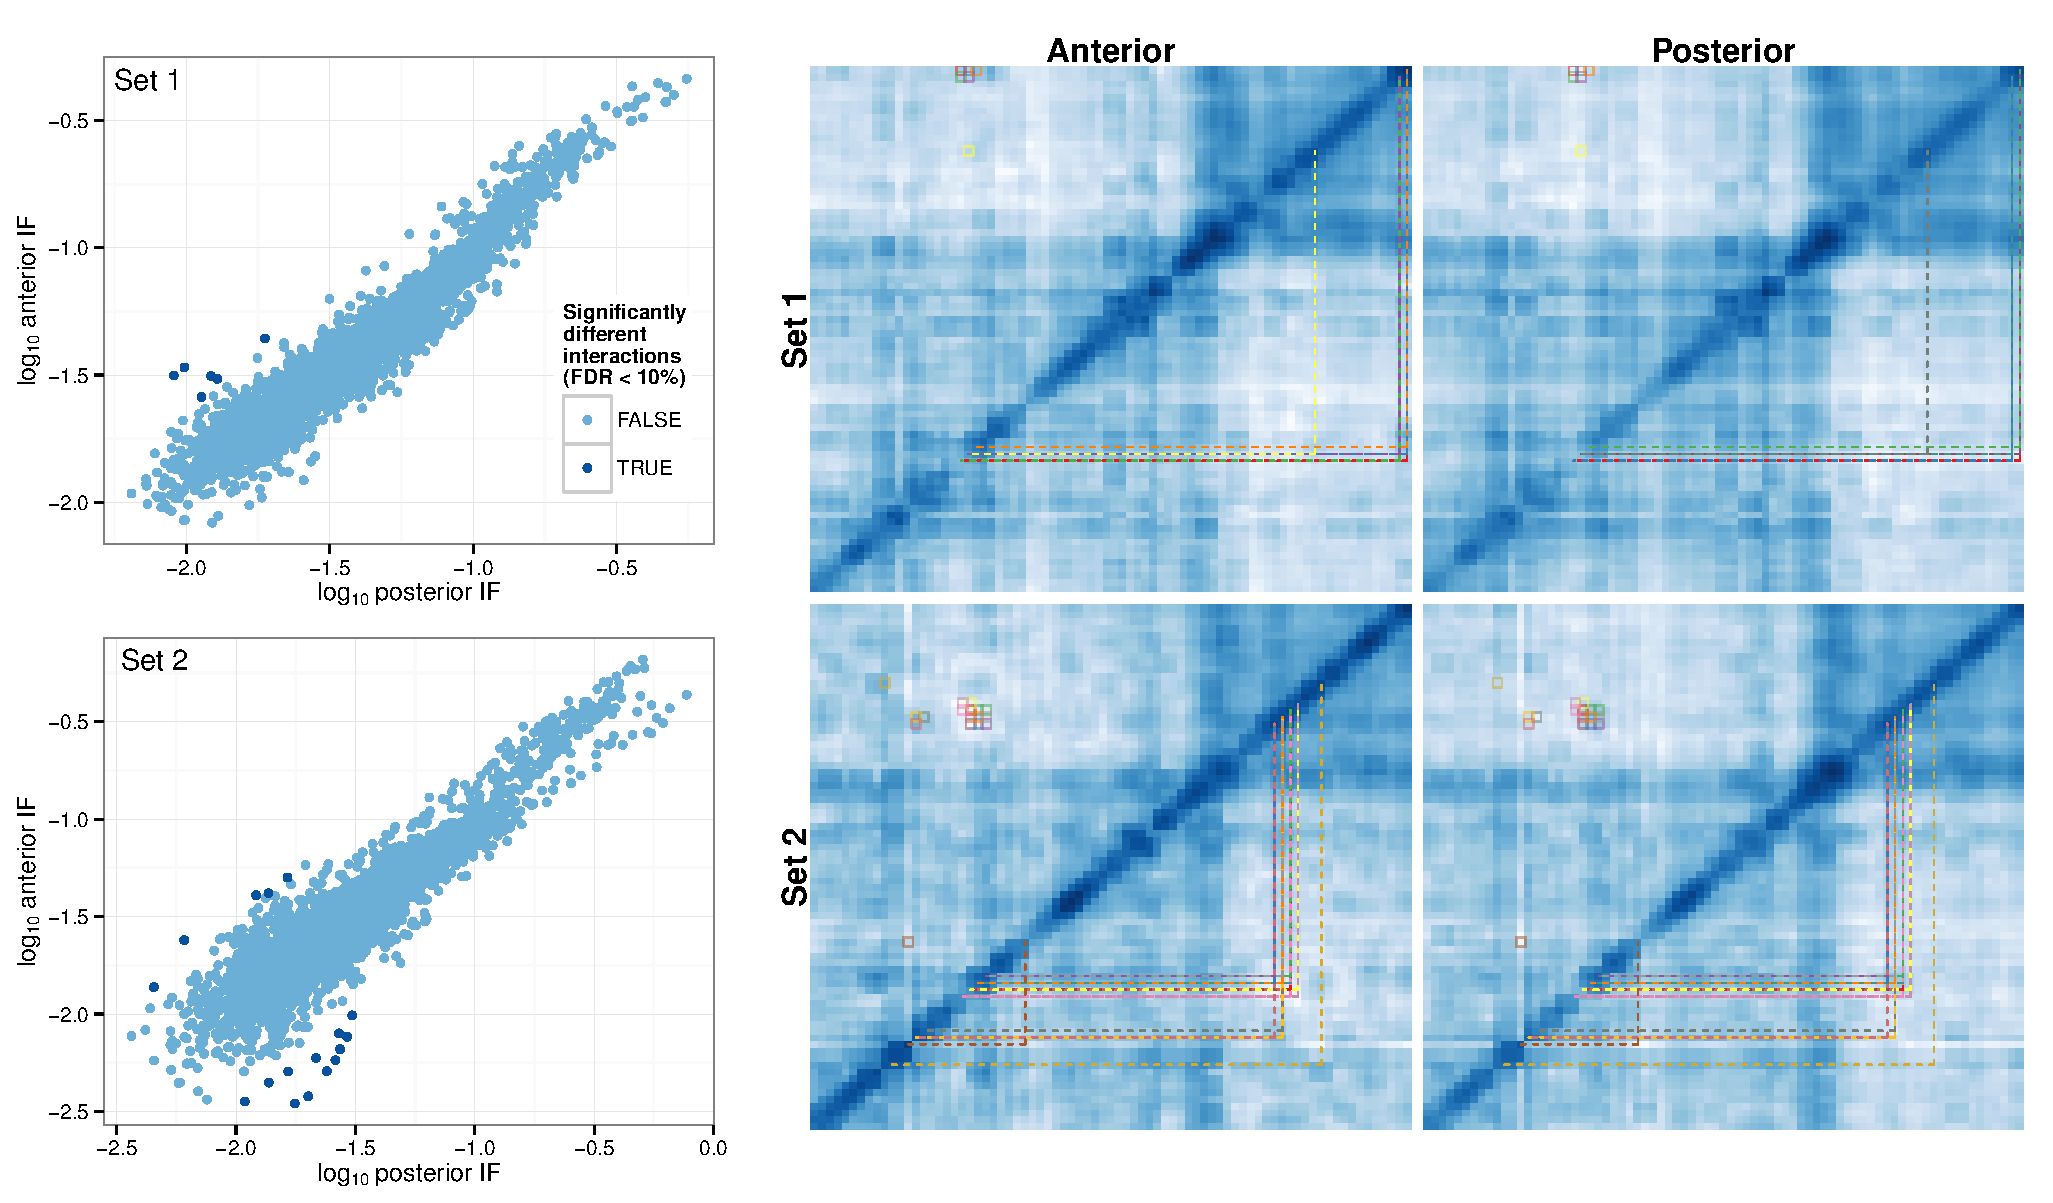
\includegraphics[width=\textwidth]{figs/5cdiff.pdf}
\captionsetup{width=\textwidth} 
\caption{ {\bf Will we use this stuff? }
Placeholder
}\label{fig:5cdiff}
\end{center} 
\end{figure} 


\subsection{5C / Hi-C comparison}

\begin{figure}
\begin{center} 
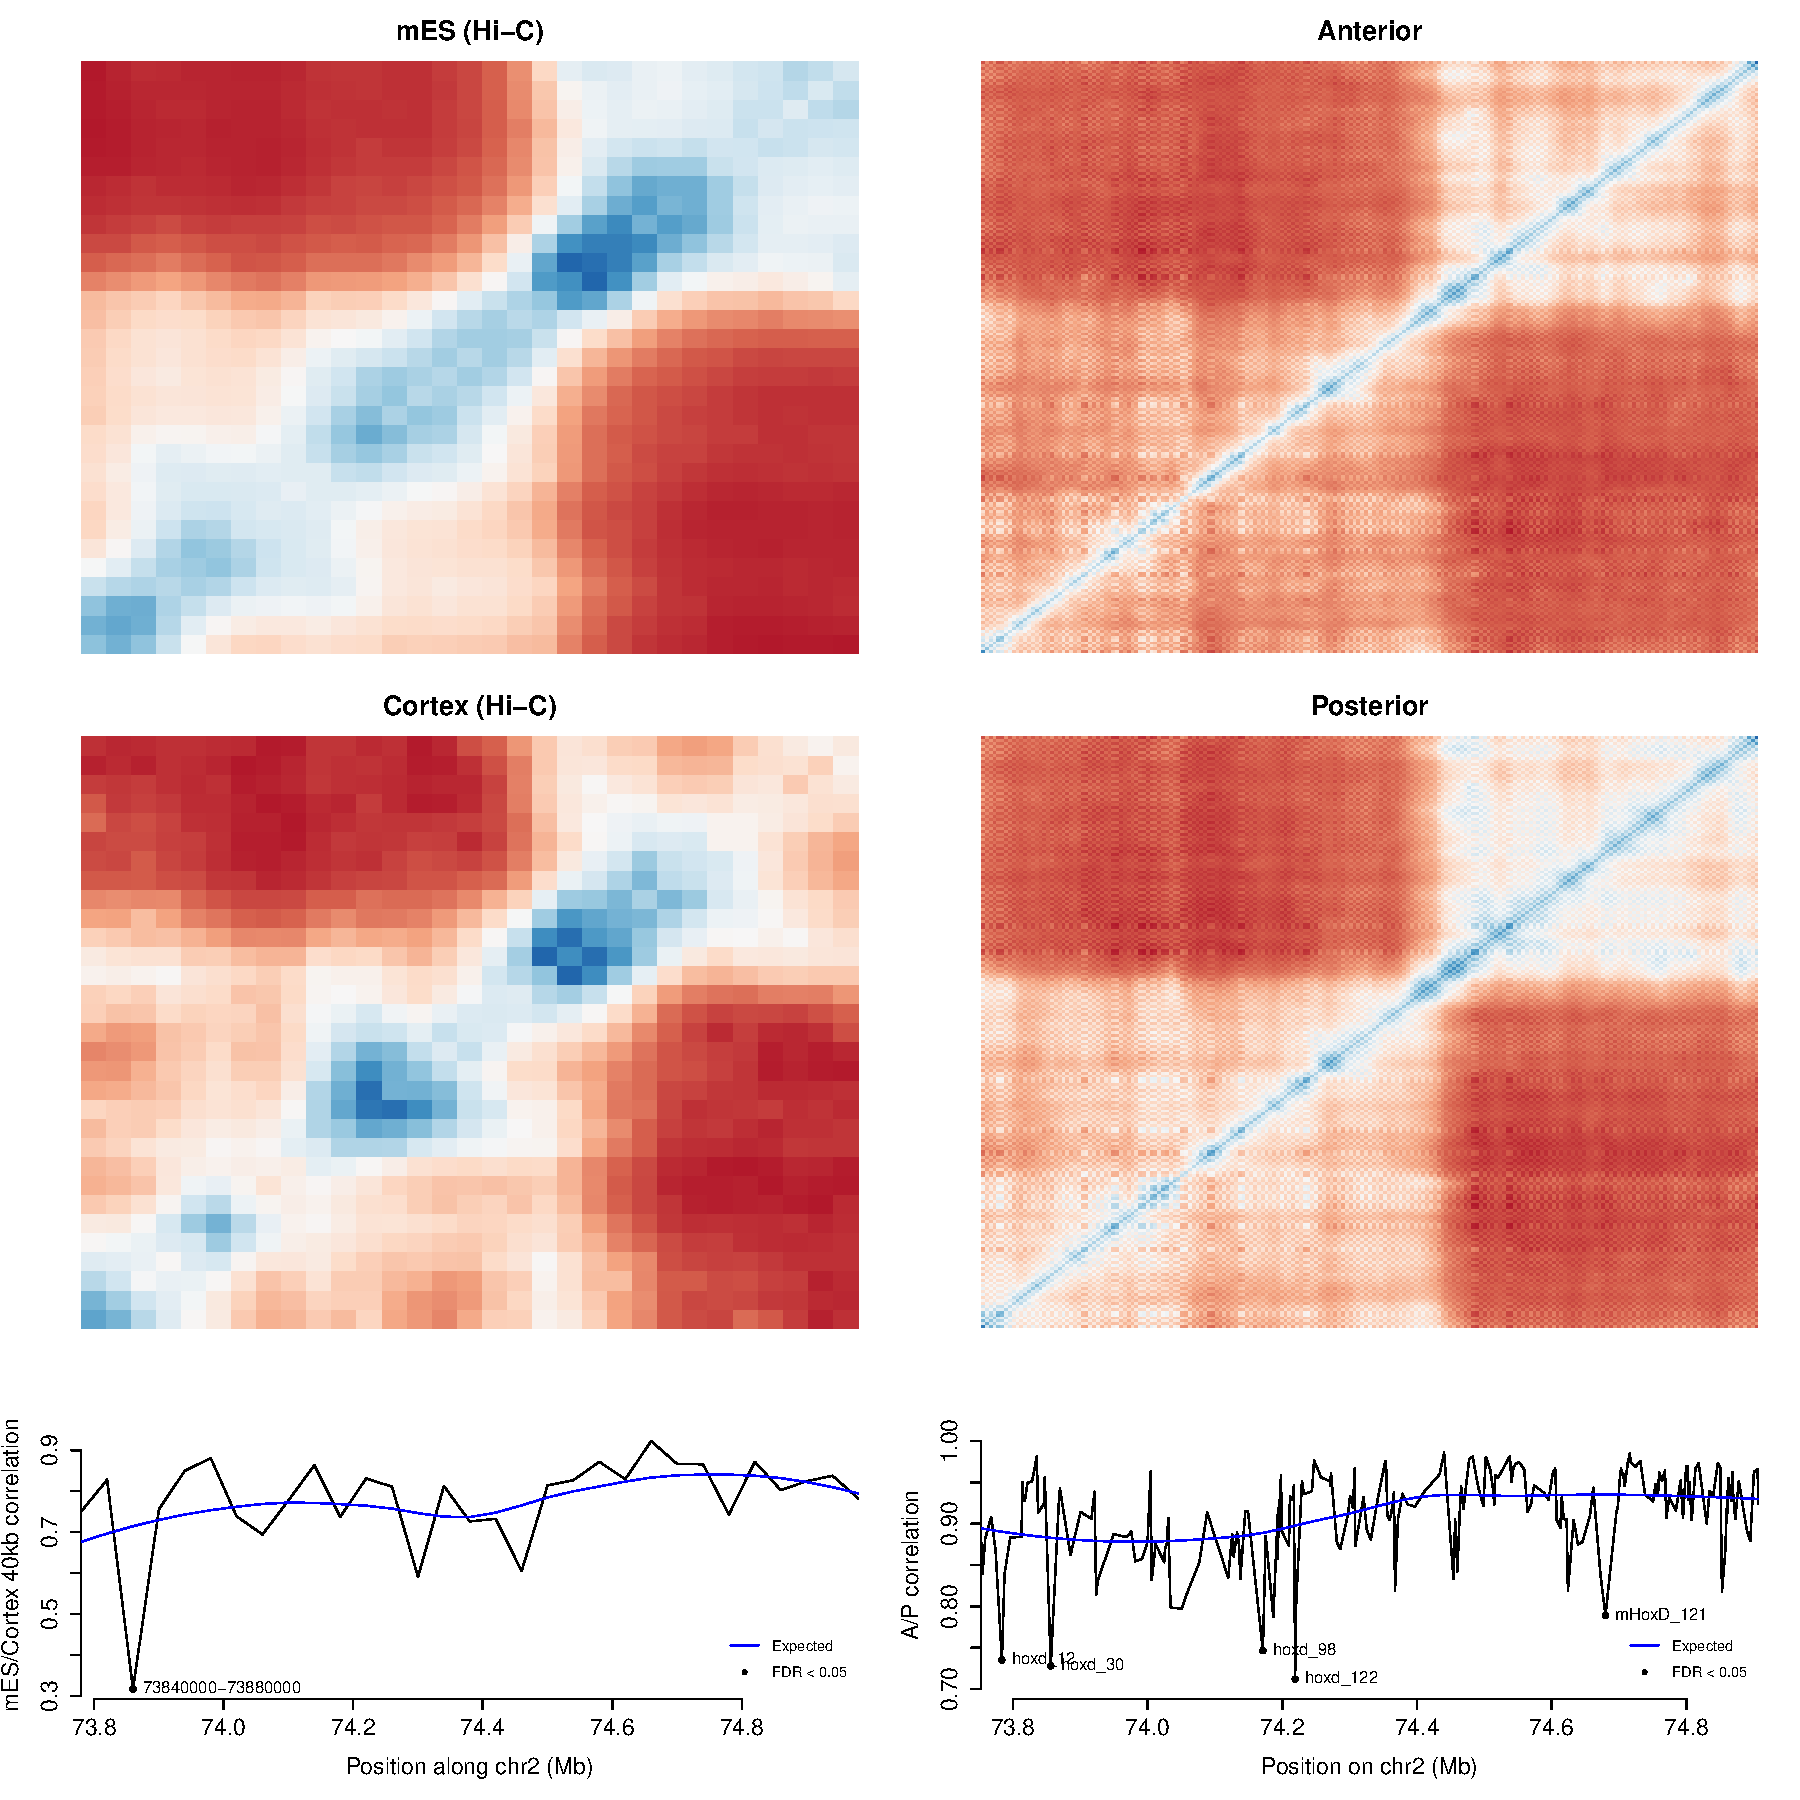
\includegraphics[width=\textwidth]{figs/5chic.pdf}
\captionsetup{width=\textwidth} 
\caption{ {\bf Will we use this stuff? }
Placeholder
}\label{fig:5cdiff}
\end{center} 
\end{figure} 


\ifstandalone
\begin{small}
\bibliography{/Users/benmoore/Documents/library,/Users/benmoore/Documents/customrefs}
\end{small}
\fi

\end{document}
